\documentclass[12pt,a4paper]{article}

% ─── Page Layout ───────────────────────────────────────────────────────────────
\usepackage[a4paper, margin=0.8in, headheight=14pt]{geometry}

% ─── Fonts (XeLaTeX) ───────────────────────────────────────────────────────────
\usepackage{fontspec}
\usepackage{unicode-math}
\setmainfont{TeX Gyre Pagella}
\setmonofont[Scale=0.88]{TeX Gyre Cursor}
\setmathfont{Latin Modern Math}

% ─── Packages ──────────────────────────────────────────────────────────────────
\usepackage{xcolor}
\usepackage{colortbl}
\usepackage{titlesec}
\usepackage{enumitem}
\usepackage{tabularx}
\usepackage{booktabs}
\usepackage{array}
\usepackage{amsmath}
\usepackage{tikz}
\usetikzlibrary{shapes.geometric, arrows.meta, positioning, calc, fit, decorations.pathreplacing, patterns}
\usepackage{tcolorbox}
\tcbuselibrary{skins, breakable}
\usepackage{hyperref}
\usepackage{fancyhdr}
\usepackage{graphicx}
\usepackage{microtype}
\hyphenpenalty=10000
\exhyphenpenalty=10000
\sloppy
\usepackage{caption}
\usepackage{setspace}
\usepackage{multirow}
\usepackage{tocloft}

% ─── Q&A helper ────────────────────────────────────────────────────────────────
\newcommand{\Q}[1]{\textbf{#1}\par\noindent\ignorespaces}

% ─── Colour Palette ────────────────────────────────────────────────────────────
\definecolor{myred}{RGB}{196,30,58}
\definecolor{mydark}{RGB}{30,30,50}
\definecolor{mygreen}{RGB}{14,120,80}
\definecolor{myteal}{RGB}{0,130,140}
\definecolor{myamber}{RGB}{180,100,0}
\definecolor{mypurple}{RGB}{100,30,160}
\definecolor{mygray}{RGB}{246,247,249}
\definecolor{mgframe}{RGB}{180,185,200}
\definecolor{watermark}{RGB}{145,150,170}
\definecolor{hdrred}{RGB}{250,232,235}
\definecolor{hdrgreen}{RGB}{220,244,233}
\definecolor{hdrteal}{RGB}{220,242,244}
\definecolor{hdramber}{RGB}{253,242,215}
\definecolor{hdrpurple}{RGB}{238,228,255}
\definecolor{hdrgray}{RGB}{238,240,245}
\definecolor{rowalt}{RGB}{250,251,253}

% ─── Section Formatting ────────────────────────────────────────────────────────
\titleformat{\section}
  {\large\bfseries\color{myred}}{\thesection.}{0.5em}{}
  [\vspace{1pt}{\color{myred}\rule{\linewidth}{0.8pt}}]
\titleformat{\subsection}
  {\normalsize\bfseries\color{myteal}}{\thesubsection}{0.5em}{}
\titlespacing*{\section}{0pt}{18pt}{7pt}
\titlespacing*{\subsection}{0pt}{11pt}{4pt}

% ─── Paragraph ─────────────────────────────────────────────────────────────────
\setlength{\parindent}{0pt}
\setlength{\parskip}{4pt}

% ─── TOC Styling ───────────────────────────────────────────────────────────────
\renewcommand{\cfttoctitlefont}{\large\bfseries\color{myred}}
\renewcommand{\cftaftertoctitle}{\par\noindent{\color{myred}\rule{\linewidth}{0.8pt}}}
\setlength{\cftbeforetoctitleskip}{0pt}
\setlength{\cftaftertoctitleskip}{6pt}
\renewcommand{\cftsecfont}{\normalsize\bfseries\color{mydark}}
\renewcommand{\cftsecpagefont}{\normalsize\bfseries\color{mydark}}
\renewcommand{\cftsecleader}{\cftdotfill{\cftdotsep}}
\setlength{\cftbeforesecskip}{7pt}
\renewcommand{\cftsubsecfont}{\small\color{mydark}}
\renewcommand{\cftsubsecpagefont}{\small\color{mydark}}
\setlength{\cftbeforesubsecskip}{3pt}
\setlength{\cftsubsecindent}{1.4em}

% ─── Table helpers ─────────────────────────────────────────────────────────────
\renewcommand{\arraystretch}{1.45}
\setlength{\tabcolsep}{6pt}
\arrayrulecolor{mydark}
\newcolumntype{B}[1]{>{\small\bfseries\raggedright\arraybackslash}m{#1}}
\newcolumntype{Y}{>{\small\raggedright\arraybackslash}X}
\renewcommand{\tabularxcolumn}[1]{m{#1}}

% ─── Header / Footer ───────────────────────────────────────────────────────────
\pagestyle{fancy}
\fancyhf{}
\fancyhead[L]{\small\color{myred}\textbf{BS-M301}\;\color{mydark}--- Probability and Statistics}
\fancyhead[R]{\small\color{myteal}\textbf{Module 2 Notes}}
\fancyfoot[C]{\small\color{mydark}\thepage}
\fancyfoot[R]{\small\color{watermark}\textit{\copyright\ Biraj}}
\renewcommand{\headrulewidth}{0.5pt}
\renewcommand{\footrulewidth}{0.3pt}

% ─── Hyperref ──────────────────────────────────────────────────────────────────
\hypersetup{
  colorlinks=true, linkcolor=myteal, urlcolor=myteal,
  pdfauthor={Biraj Sarkar (CGEC)},
  pdftitle={BS-M301 --- Module 2 Notes: Continuous Probability Distributions}
}

% ─── tcolorbox styles ──────────────────────────────────────────────────────────
\tcbset{
  tikzbox/.style={
    colback=mygray, colframe=mgframe, boxrule=0.6pt, arc=4pt,
    left=8pt, right=8pt, top=6pt, bottom=6pt,
    colbacktitle=mgframe, coltitle=mydark,
    fonttitle=\small\bfseries
  },
  defbox/.style={
    colback=hdrgreen, colframe=mygreen, boxrule=0.8pt, arc=4pt,
    left=9pt, right=9pt, top=6pt, bottom=6pt,
    colbacktitle=mygreen, coltitle=white,
    fonttitle=\small\bfseries
  },
  formulabox/.style={
    colback=hdrteal, colframe=myteal, boxrule=0.8pt, arc=4pt,
    left=9pt, right=9pt, top=7pt, bottom=7pt,
    colbacktitle=myteal, coltitle=white,
    fonttitle=\small\bfseries
  },
  examplebox/.style={
    colback=hdramber, colframe=myamber, boxrule=0.8pt, arc=4pt,
    left=9pt, right=9pt, top=6pt, bottom=6pt,
    colbacktitle=myamber, coltitle=white,
    fonttitle=\small\bfseries
  },
  masonbox/.style={
    colback=hdrpurple, colframe=mypurple, boxrule=0.8pt, arc=4pt,
    left=9pt, right=9pt, top=6pt, bottom=6pt,
    colbacktitle=mypurple, coltitle=white,
    fonttitle=\small\bfseries
  },
  exambox/.style={
    colback=hdrpurple, colframe=mypurple, boxrule=1pt, arc=5pt,
    left=10pt, right=10pt, top=8pt, bottom=8pt,
    colbacktitle=mypurple, coltitle=white,
    fonttitle=\bfseries,
    breakable, title after break={\textbf{Frequently Asked / Viva Questions (contd.)}}
  }
}
\tcbset{breakable}
\tcbset{after={\color{black}}}

% ─── TikZ styles ───────────────────────────────────────────────────────────────
\tikzset{
  arrow/.style={-Stealth, thick, color=mydark},
  redarrow/.style={-Stealth, thick, color=myred},
  line/.style={thick, color=mydark}
}

\begin{document}

% ─── Title Page ───────────────────────────────────────────────────────────────
\begin{center}
  {\LARGE\bfseries\color{myred} BS-M301 --- Probability and Statistics}\\[5pt]
  {\normalsize\color{mydark} Semester III \quad$\bullet$\quad 3L:0T:3P \quad$\bullet$\quad 3 Credits}\\[3pt]
  {\normalsize\color{myteal}\textbf{Module 2 Exam Notes: Continuous Probability Distributions}}\\[3pt]
  {\small\color{mydark} CGEC \;$|$\; B.Tech ECE (2023--27) \;$|$\; \textit{Biraj Sarkar}}
\end{center}
\vspace{2pt}
\noindent{\color{myred}\rule{\linewidth}{1.5pt}}
\vspace{2pt}

\hypersetup{linkcolor=mydark}
\tableofcontents
\hypersetup{linkcolor=myteal}
\newpage

% ───────────────────────────────────────────────────────────────────────────────
\section{Continuous Random Variables, PDF and CDF}
% ───────────────────────────────────────────────────────────────────────────────

A random variable is classified as \textbf{continuous} if its range consists of an entire interval or a union of intervals on the real line $\mathbb{R}$ (such as voltage, time, temperature, or noise amplitude). Because an interval contains uncountably infinitely many points, the probability that a continuous random variable assumes any exact single real value is strictly zero: $P(X = c) = 0$ for every $c \in \mathbb{R}$.

\begin{tcolorbox}[defbox, title={\textbf{Definition: Probability Density Function (PDF)}}]
A function $f_X: \mathbb{R} \to \mathbb{R}$ is called the \textbf{Probability Density Function (PDF)} of a continuous random variable $X$ if for any interval $[a, b] \subseteq \mathbb{R}$:
\begin{equation}
  P(a \le X \le b) = \int_a^b f_X(x) \, dx
\end{equation}
Every valid PDF must strictly satisfy two axiomatic criteria:
\begin{align}
  \textbf{Non-negativity:} \quad & f_X(x) \ge 0, \quad \forall x \in \mathbb{R} \\[4pt]
  \textbf{Total Normalization:} \quad & \int_{-\infty}^\infty f_X(x) \, dx = 1
\end{align}
\textit{Crucial Insight:} The value $f_X(x)$ represents probability \textit{density} per unit length, not probability itself! Consequently, $f_X(x)$ can exceed $1$ over narrow intervals, provided the total area under the curve equals unity.
\end{tcolorbox}

\subsection{Cumulative Distribution Function (CDF)}
The \textbf{Cumulative Distribution Function (CDF)} of a continuous random variable $X$ is defined as the area under the PDF curve from $-\infty$ up to threshold $x$:
\begin{equation}
  F_X(x) = P(X \le x) = \int_{-\infty}^x f_X(t) \, dt
\end{equation}
By the Fundamental Theorem of Calculus, at every point where $f_X(x)$ is continuous, the PDF is the exact first derivative of the CDF:
\begin{equation}
  f_X(x) = \frac{d}{dx} F_X(x)
\end{equation}

\begin{tcolorbox}[formulabox, title={\textbf{Key Properties of Continuous CDF and Interval Probabilities}}]
\begin{enumerate}[leftmargin=*, itemsep=3pt]
  \item \textbf{Continuous and Smooth:} Unlike discrete CDFs (which have jump discontinuities), the CDF $F_X(x)$ of a continuous random variable is everywhere continuous.
  \item \textbf{Boundary Limits:} $\displaystyle\lim_{x \to -\infty} F_X(x) = 0$ and $\displaystyle\lim_{x \to +\infty} F_X(x) = 1$.
  \item \textbf{Boundary Invariance of Interval Probabilities:} Since single-point probabilities are zero ($P(X = a) = P(X = b) = 0$):
  \begin{align}
    P(a < X < b) &= P(a \le X < b) = P(a < X \le b) = P(a \le X \le b) \nonumber \\[2pt]
                 &= F_X(b) - F_X(a) = \int_a^b f_X(x) \, dx
  \end{align}
  \item \textbf{Tail (Survival) Function:} $R_X(x) = P(X > x) = 1 - F_X(x) = \int_x^\infty f_X(t) \, dt$.
\end{enumerate}
\end{tcolorbox}

\subsection{Expectation, Variance and Moment Generating Function (MGF)}
\begin{itemize}[leftmargin=*, itemsep=3pt]
  \item \textbf{Mathematical Expectation (Mean):}
  \begin{equation}
    \mu = E[X] = \int_{-\infty}^\infty x f_X(x) \, dx \quad (\text{provided } \int_{-\infty}^\infty |x| f_X(x) dx < \infty)
  \end{equation}
  \item \textbf{Variance ($\sigma^2$):}
  \begin{equation}
    \operatorname{Var}(X) = \sigma^2 = \int_{-\infty}^\infty (x - \mu)^2 f_X(x) \, dx = E[X^2] - (E[X])^2
  \end{equation}
  \item \textbf{Moment Generating Function (MGF):} The MGF $M_X(t)$ is defined as the Laplace-type transform:
  \begin{equation}
    M_X(t) = E\left[e^{tX}\right] = \int_{-\infty}^\infty e^{tx} f_X(x) \, dx
  \end{equation}
  provided the integral converges in an open neighborhood around $t = 0$ ($|t| < h$).
  \item \textbf{Generation of Moments from MGF:} Expanding $e^{tX} = \sum_{r=0}^\infty \frac{t^r X^r}{r!}$:
  \begin{equation}
    M_X(t) = \sum_{r=0}^\infty \frac{t^r}{r!} E[X^r] = 1 + \mu_1' t + \frac{\mu_2' t^2}{2!} + \frac{\mu_3' t^3}{3!} + \cdots
  \end{equation}
  Differentiating $r$ times and setting $t = 0$:
  \begin{equation}
    \mu_r' = E[X^r] = \left.\frac{d^r M_X(t)}{dt^r}\right|_{t=0}
  \end{equation}
\end{itemize}

% ───────────────────────────────────────────────────────────────────────────────
\section{The Normal (Gaussian) Distribution}
% ───────────────────────────────────────────────────────────────────────────────

The \textbf{Normal distribution} (discovered by Carl Friedrich Gauss) is the central pillar of engineering probability, signal analysis, and statistics. By the Central Limit Theorem, the sum of a large number of independent random disturbances converges to a normal distribution, regardless of the underlying distribution of the individual components.

\begin{tcolorbox}[defbox, title={\textbf{Definition: Normal Distribution $\mathcal{N}(\mu, \sigma^2)$}}]
A continuous random variable $X$ has a \textbf{Normal distribution} with mean $\mu \in \mathbb{R}$ and variance $\sigma^2 > 0$ (written $X \sim \mathcal{N}(\mu, \sigma^2)$) if its PDF is:
\begin{equation}
  f_X(x) = \frac{1}{\sigma\sqrt{2\pi}} \exp\left(-\frac{(x - \mu)^2}{2\sigma^2}\right), \qquad -\infty < x < \infty
\end{equation}
\end{tcolorbox}

\subsection{Mathematical Verification of the Normalizing Constant}
To verify $\int_{-\infty}^\infty f_X(x) dx = 1$, let $I = \int_{-\infty}^\infty \frac{1}{\sigma\sqrt{2\pi}} e^{-(x-\mu)^2/(2\sigma^2)} dx$.
Substitute the standard normal transform $z = \frac{x - \mu}{\sigma} \implies dx = \sigma dz$:
\begin{equation}
  I = \frac{1}{\sqrt{2\pi}} \int_{-\infty}^\infty e^{-z^2/2} \, dz
\end{equation}
Let $J = \int_{-\infty}^\infty e^{-z^2/2} dz$. Converting $J^2$ to polar coordinates ($x = r\cos\theta, y = r\sin\theta, dx dy = r dr d\theta$):
\begin{equation}
  J^2 = \int_{-\infty}^\infty e^{-x^2/2} dx \int_{-\infty}^\infty e^{-y^2/2} dy = \int_0^{2\pi} d\theta \int_0^\infty r e^{-r^2/2} \, dr = 2\pi \left[-e^{-r^2/2}\right]_0^\infty = 2\pi(1) = 2\pi
\end{equation}
Hence $J = \sqrt{2\pi}$, confirming $I = \frac{1}{\sqrt{2\pi}} \cdot \sqrt{2\pi} = 1$.

\begin{tcolorbox}[examplebox, title={\textbf{Derivation: MGF and Moments of the Normal Distribution}}]
For $X \sim \mathcal{N}(\mu, \sigma^2)$, the MGF is:
\begin{equation}
  M_X(t) = E[e^{tX}] = \int_{-\infty}^\infty e^{tx} \cdot \frac{1}{\sigma\sqrt{2\pi}} e^{-(x-\mu)^2/(2\sigma^2)} \, dx
\end{equation}
Substituting $z = \frac{x-\mu}{\sigma} \implies x = \mu + \sigma z$ and $dx = \sigma dz$:
\begin{align}
  M_X(t) &= \frac{1}{\sqrt{2\pi}} \int_{-\infty}^\infty e^{t(\mu + \sigma z)} e^{-z^2/2} \, dz = e^{\mu t} \cdot \frac{1}{\sqrt{2\pi}} \int_{-\infty}^\infty \exp\left(-\frac{1}{2}(z^2 - 2\sigma t z)\right) dz
\end{align}
Completing the square in the exponent: $z^2 - 2\sigma t z = (z - \sigma t)^2 - \sigma^2 t^2$:
\begin{equation}
  M_X(t) = e^{\mu t} e^{\sigma^2 t^2 / 2} \cdot \underbrace{\frac{1}{\sqrt{2\pi}} \int_{-\infty}^\infty e^{-(z - \sigma t)^2/2} \, dz}_{= 1 \text{ (integral of standard normal density)}} = \exp\left(\mu t + \frac{1}{2}\sigma^2 t^2\right)
\end{equation}
\textbf{Moments via Derivatives of MGF:}
\begin{align}
  M_X'(t) &= (\mu + \sigma^2 t) e^{\mu t + \frac{1}{2}\sigma^2 t^2} \implies E[X] = M_X'(0) = \mu \\[3pt]
  M_X''(t) &= \left[\sigma^2 + (\mu + \sigma^2 t)^2\right] e^{\mu t + \frac{1}{2}\sigma^2 t^2} \implies E[X^2] = M_X''(0) = \sigma^2 + \mu^2 \\[3pt]
  \operatorname{Var}(X) &= E[X^2] - (E[X])^2 = (\sigma^2 + \mu^2) - \mu^2 = \sigma^2
\end{align}
\end{tcolorbox}

\subsection{Symmetry, Odd Moments and Inflection Points}
\begin{enumerate}[leftmargin=*, itemsep=3pt]
  \item \textbf{Symmetry about $\mu$:} The bell curve is symmetric about the vertical line $x = \mu$: $f_X(\mu - x) = f_X(\mu + x)$. Consequently:
  \begin{equation}
    \text{Mean} = \text{Median} = \text{Mode} = \mu
  \end{equation}
  \item \textbf{Vanishing of All Odd Central Moments:} By anti-symmetry of odd powers about zero:
  \begin{equation}
    \mu_{2k+1} = E[(X - \mu)^{2k+1}] = \int_{-\infty}^\infty (x-\mu)^{2k+1} f_X(x) \, dx = 0 \quad \forall k \in \mathbb{N}_0
  \end{equation}
  Specifically $\mu_1 = 0$ and $\mu_3 = 0$. Hence the skewness coefficient is identically zero: $\beta_1 = \gamma_1 = 0$.
  \item \textbf{Even Central Moments and Kurtosis:}
  \begin{equation}
    \mu_{2k} = 1 \cdot 3 \cdot 5 \cdots (2k-1) \, \sigma^{2k} = \frac{(2k)!}{2^k k!} \sigma^{2k} \implies \mu_4 = 3\sigma^4
  \end{equation}
  The coefficient of kurtosis is: $\beta_2 = \frac{\mu_4}{\mu_2^2} = \frac{3\sigma^4}{(\sigma^2)^2} = 3$ (Mesokurtic benchmark).
  \item \textbf{Points of Inflection:} Finding where the concavity changes ($\frac{d^2 f_X}{dx^2} = 0$):
  \begin{align}
    f_X'(x) &= -\frac{x - \mu}{\sigma^2} f_X(x) \\[2pt]
    f_X''(x) &= \left[\left(\frac{x - \mu}{\sigma^2}\right)^2 - \frac{1}{\sigma^2}\right] f_X(x) = 0 \implies (x - \mu)^2 = \sigma^2 \implies x = \mu \pm \sigma
  \end{align}
  The curve shifts from concave-downward to concave-upward at exactly $x = \mu \pm \sigma$.
\end{enumerate}

\begin{tcolorbox}[tikzbox, title={\textbf{TikZ Schematic: Standard Normal Gaussian Curve with Inflection Points and Area Rules}}]
\begin{center}
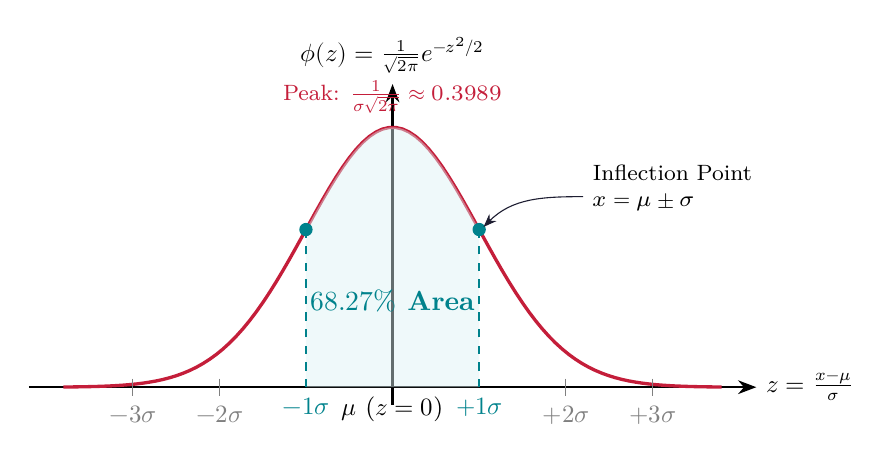
\begin{tikzpicture}[scale=1.1, every node/.style={font=\small}]
  % Axes
  \draw[-Stealth, thick] (-4.2, 0) -- (4.2, 0) node[right] {$z = \frac{x-\mu}{\sigma}$};
  \draw[-Stealth, thick] (0, -0.2) -- (0, 3.5) node[above] {$\phi(z) = \frac{1}{\sqrt{2\pi}} e^{-z^2/2}$};

  % Bell curve formula plot
  % Peak at z=0 is 1/sqrt(2pi) = 0.3989 -> scaled by 7.5 gives y = 3.0
  \draw[very thick, color=myred, domain=-3.8:3.8, samples=100]
    plot (\x, {3.0*exp(-(\x)^2/2)});

  % Shading 1-sigma central zone
  \fill[fill=hdrteal, fill opacity=0.45, domain=-1:1, samples=60]
    (-1,0) -- plot (\x, {3.0*exp(-(\x)^2/2)}) -- (1,0) -- cycle;

  % Inflection point markers at z = -1 and z = +1
  % Height at z=1 is 3.0*exp(-0.5) = 1.82
  \draw[thick, dashed, color=myteal] (-1, 0) node[below] {$-1\sigma$} -- (-1, 1.82);
  \filldraw[color=myteal] (-1, 1.82) circle (2pt);

  \draw[thick, dashed, color=myteal] (1, 0) node[below] {$+1\sigma$} -- (1, 1.82);
  \filldraw[color=myteal] (1, 1.82) circle (2pt);

  % 2-sigma and 3-sigma tick markers
  \draw[thin, color=gray] (-2, 0.1) -- (-2, -0.1) node[below] {$-2\sigma$};
  \draw[thin, color=gray] (2, 0.1) -- (2, -0.1) node[below] {$+2\sigma$};
  \draw[thin, color=gray] (-3, 0.1) -- (-3, -0.1) node[below] {$-3\sigma$};
  \draw[thin, color=gray] (3, 0.1) -- (3, -0.1) node[below] {$+3\sigma$};
  \node[below] at (0, 0) {$\mu$ ($z=0$)};

  % Annotations
  \node[color=myteal, font=\bfseries] at (0, 1.0) {$68.27\%$ Area};
  \node[above, color=myred, font=\footnotesize] at (0, 3.05) {Peak: $\frac{1}{\sigma\sqrt{2\pi}} \approx 0.3989$};

  \draw[-Stealth, thin, color=mydark] (2.2, 2.2) to[out=180, in=45] (1.05, 1.85);
  \node[right, font=\footnotesize, align=left] at (2.2, 2.3) {Inflection Point\\$x = \mu \pm \sigma$};
\end{tikzpicture}
\end{center}
\end{tcolorbox}

\subsection{Standard Normal Distribution and \texorpdfstring{$\Phi(z)$}{Phi(z)} Function}
When $\mu = 0$ and $\sigma = 1$, the variable is denoted $Z \sim \mathcal{N}(0, 1)$ with standard normal PDF $\phi(z) = \frac{1}{\sqrt{2\pi}} e^{-z^2/2}$ and CDF:
\begin{equation}
  \Phi(z) = P(Z \le z) = \frac{1}{\sqrt{2\pi}} \int_{-\infty}^z e^{-u^2/2} \, du
\end{equation}
By symmetry:
\begin{equation}
  \Phi(-z) = 1 - \Phi(z) \qquad \text{and} \qquad P(a \le X \le b) = \Phi\left(\frac{b - \mu}{\sigma}\right) - \Phi\left(\frac{a - \mu}{\sigma}\right)
\end{equation}

% ───────────────────────────────────────────────────────────────────────────────
\section{The Exponential Distribution}
% ───────────────────────────────────────────────────────────────────────────────

The \textbf{Exponential distribution} models the continuous time elapsed between independent random events occurring at a constant average rate $\lambda > 0$ (such as service times, component lifetimes, and inter-arrival times in queueing systems).

\begin{tcolorbox}[defbox, title={\textbf{Definition: Exponential Distribution $\mathbf{Exp(\lambda)}$}}]
A continuous random variable $X$ has an \textbf{Exponential distribution} with rate parameter $\lambda > 0$ ($X \sim \text{Exp}(\lambda)$) if its PDF is:
\begin{equation}
  f_X(x) =
  \begin{cases}
    \lambda e^{-\lambda x}, & x \ge 0 \\[3pt]
    0, & x < 0
  \end{cases}
\end{equation}
\end{tcolorbox}

\subsection{Derivation of CDF, Mean, Variance and MGF}
\begin{enumerate}[leftmargin=*, itemsep=3pt]
  \item \textbf{Cumulative Distribution Function (CDF):} For $x \ge 0$:
  \begin{equation}
    F_X(x) = \int_0^x \lambda e^{-\lambda t} \, dt = \left[-e^{-\lambda t}\right]_0^x = 1 - e^{-\lambda x}
  \end{equation}
  The survival (tail) probability is:
  \begin{equation}
    P(X > x) = 1 - F_X(x) = e^{-\lambda x}
  \end{equation}
  \item \textbf{Moment Generating Function (MGF):} For $t < \lambda$:
  \begin{equation}
    M_X(t) = \int_0^\infty e^{tx} \lambda e^{-\lambda x} \, dx = \lambda \int_0^\infty e^{-(\lambda - t)x} \, dx = \frac{\lambda}{\lambda - t} = \left(1 - \frac{t}{\lambda}\right)^{-1}
  \end{equation}
  Expanding in powers of $t/\lambda$:
  \begin{equation}
    M_X(t) = 1 + \frac{t}{\lambda} + \frac{t^2}{\lambda^2} + \frac{t^3}{\lambda^3} + \cdots = 1 + \left(\frac{1}{\lambda}\right) t + \left(\frac{2}{\lambda^2}\right) \frac{t^2}{2!} + \cdots
  \end{equation}
  \item \textbf{Mean and Variance:}
  \begin{equation}
    \mu = E[X] = \frac{1}{\lambda}, \qquad E[X^2] = \frac{2}{\lambda^2} \implies \operatorname{Var}(X) = E[X^2] - (E[X])^2 = \frac{2}{\lambda^2} - \frac{1}{\lambda^2} = \frac{1}{\lambda^2}
  \end{equation}
  Standard deviation is $\sigma = \frac{1}{\lambda}$. Notice that for the Exponential distribution: $\sigma = \mu$.
\end{enumerate}

\subsection{The Memoryless Property (Markov Property)}
\begin{tcolorbox}[examplebox, title={\textbf{Theorem: Memoryless Property of the Exponential Distribution}}]
Let $X \sim \text{Exp}(\lambda)$. For any non-negative time increments $s, t \ge 0$:
\begin{equation}
  P(X > s + t \mid X > s) = P(X > t)
\end{equation}
\textbf{Proof:} Using the conditional probability definition and $P(X > x) = e^{-\lambda x}$:
\begin{align}
  P(X > s + t \mid X > s) &= \frac{P(\{X > s + t\} \cap \{X > s\})}{P(X > s)} \nonumber \\[4pt]
                          &= \frac{P(X > s + t)}{P(X > s)} = \frac{e^{-\lambda(s+t)}}{e^{-\lambda s}} = \frac{e^{-\lambda s} e^{-\lambda t}}{e^{-\lambda s}} = e^{-\lambda t} = P(X > t)
\end{align}
\textit{Physical Interpretation:} If a semiconductor component has survived $s$ hours without failing, the probability that it survives an additional $t$ hours is identical to the probability that a brand-new component survives $t$ hours. The component suffers no wear-out aging over time!
\end{tcolorbox}

\begin{tcolorbox}[tikzbox, title={\textbf{TikZ Plot: Exponential Probability Density Functions for Different Rates $\lambda$}}]
\begin{center}
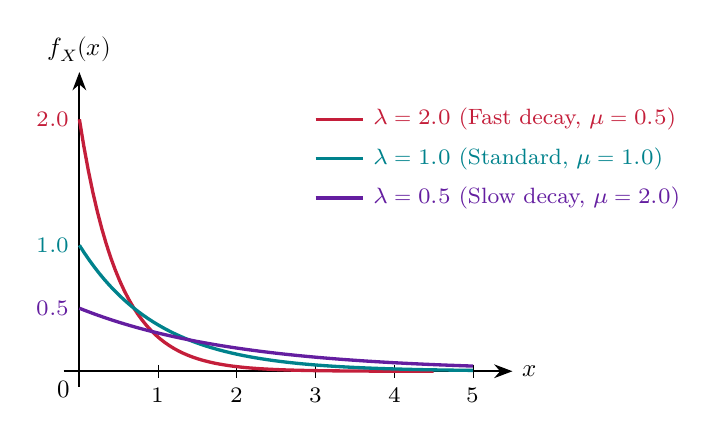
\begin{tikzpicture}[scale=1.0, every node/.style={font=\small}]
  % Axes
  \draw[-Stealth, thick] (-0.2, 0) -- (5.5, 0) node[right] {$x$};
  \draw[-Stealth, thick] (0, -0.2) -- (0, 3.8) node[above] {$f_X(x)$};

  % Ticks
  \foreach \x in {1,2,3,4,5} {
    \draw (\x, 0.08) -- (\x, -0.08) node[below] {\footnotesize $\x$};
  }
  \node[below left] at (0,0) {$0$};

  % Curves:
  % lambda = 2.0: peak at (0, 3.2), scale: 2.0 -> y=3.2
  \draw[very thick, color=myred, domain=0:4.5, samples=80]
    plot (\x, {3.2*exp(-2.0*\x)});
  \node[left, color=myred] at (0, 3.2) {\footnotesize $2.0$};

  % lambda = 1.0: peak at (0, 1.6)
  \draw[very thick, color=myteal, domain=0:5.0, samples=80]
    plot (\x, {1.6*exp(-1.0*\x)});
  \node[left, color=myteal] at (0, 1.6) {\footnotesize $1.0$};

  % lambda = 0.5: peak at (0, 0.8)
  \draw[very thick, color=mypurple, domain=0:5.0, samples=80]
    plot (\x, {0.8*exp(-0.5*\x)});
  \node[left, color=mypurple] at (0, 0.8) {\footnotesize $0.5$};

  % Legend
  \draw[very thick, color=myred] (3.0, 3.2) -- (3.6, 3.2) node[right, font=\footnotesize] {$\lambda = 2.0$ (Fast decay, $\mu=0.5$)};
  \draw[very thick, color=myteal] (3.0, 2.7) -- (3.6, 2.7) node[right, font=\footnotesize] {$\lambda = 1.0$ (Standard, $\mu=1.0$)};
  \draw[very thick, color=mypurple] (3.0, 2.2) -- (3.6, 2.2) node[right, font=\footnotesize] {$\lambda = 0.5$ (Slow decay, $\mu=2.0$)};
\end{tikzpicture}
\end{center}
\end{tcolorbox}

% ───────────────────────────────────────────────────────────────────────────────
\section{The Gamma Distribution and Its Properties}
% ───────────────────────────────────────────────────────────────────────────────

The \textbf{Gamma distribution} is a versatile two-parameter continuous distribution that extends the exponential distribution to model the waiting time until the occurrence of $\alpha$ successive Poisson events, as well as lifetime data exhibiting wear-out characteristics.

\begin{tcolorbox}[defbox, title={\textbf{Definition: The Gamma Function $\Gamma(\alpha)$}}]
The complete \textbf{Eulerian Gamma Function} is defined for all $\alpha > 0$ by the improper definite integral:
\begin{equation}
  \Gamma(\alpha) = \int_0^\infty u^{\alpha - 1} e^{-u} \, du
\end{equation}
\textbf{Fundamental Properties of $\Gamma(\alpha)$:}
\begin{enumerate}[leftmargin=*, itemsep=2pt]
  \item \textbf{Recurrence Relation:} $\Gamma(\alpha + 1) = \alpha \Gamma(\alpha)$ (integrating by parts).
  \item \textbf{Integer Factorial:} For any positive integer $n \in \mathbb{N}$: $\Gamma(n) = (n - 1)!$ with $\Gamma(1) = 0! = 1$.
  \item \textbf{Half-Integer Values:} $\Gamma\left(\frac{1}{2}\right) = \sqrt{\pi}$, from which $\Gamma\left(\frac{3}{2}\right) = \frac{1}{2}\sqrt{\pi}, \; \Gamma\left(\frac{5}{2}\right) = \frac{3}{4}\sqrt{\pi}$.
\end{enumerate}
\end{tcolorbox}

\begin{tcolorbox}[formulabox, title={\textbf{Two-Parameter Gamma Density $\mathbf{Gamma(\alpha, \beta)}$}}]
A random variable $X$ follows a \textbf{Gamma distribution} with shape parameter $\alpha > 0$ and rate parameter $\beta > 0$ (scale parameter $\theta = 1/\beta$) if its PDF is:
\begin{equation}
  f_X(x) =
  \begin{cases}
    \dfrac{\beta^\alpha}{\Gamma(\alpha)} x^{\alpha - 1} e^{-\beta x}, & x > 0 \\[8pt]
    0, & x \le 0
  \end{cases}
\end{equation}
\end{tcolorbox}

\subsection{Derivation of Mean, Variance and MGF of Gamma Distribution}
\begin{tcolorbox}[examplebox, title={\textbf{Rigorous Derivation: Moments of Gamma Distribution}}]
Using the MGF definition for $t < \beta$:
\begin{align}
  M_X(t) = \int_0^\infty e^{tx} \cdot \frac{\beta^\alpha}{\Gamma(\alpha)} x^{\alpha-1} e^{-\beta x} \, dx = \frac{\beta^\alpha}{\Gamma(\alpha)} \int_0^\infty x^{\alpha-1} e^{-(\beta - t)x} \, dx
\end{align}
Substitute $u = (\beta - t)x \implies x = \frac{u}{\beta - t}$ and $dx = \frac{du}{\beta - t}$:
\begin{equation}
  M_X(t) = \frac{\beta^\alpha}{\Gamma(\alpha)} \int_0^\infty \left(\frac{u}{\beta - t}\right)^{\alpha-1} e^{-u} \frac{du}{\beta - t} = \frac{\beta^\alpha}{(\beta - t)^\alpha} \cdot \underbrace{\frac{1}{\Gamma(\alpha)} \int_0^\infty u^{\alpha-1} e^{-u} du}_{= 1} = \left(1 - \frac{t}{\beta}\right)^{-\alpha}
\end{equation}
Expanding $(1 - t/\beta)^{-\alpha}$ using the generalized binomial theorem:
\begin{align}
  M_X(t) &= 1 + (-\alpha)\left(-\frac{t}{\beta}\right) + \frac{(-\alpha)(-\alpha-1)}{2!} \left(-\frac{t}{\beta}\right)^2 + \cdots \nonumber \\[3pt]
         &= 1 + \left(\frac{\alpha}{\beta}\right) t + \frac{\alpha(\alpha+1)}{\beta^2} \frac{t^2}{2!} + \cdots
\end{align}
Equating coefficients of $t$ and $t^2/2!$:
\begin{align}
  E[X] &= \mu = \frac{\alpha}{\beta} \\[3pt]
  E[X^2] &= \frac{\alpha(\alpha+1)}{\beta^2} \implies \operatorname{Var}(X) = E[X^2] - (E[X])^2 = \frac{\alpha^2 + \alpha}{\beta^2} - \frac{\alpha^2}{\beta^2} = \frac{\alpha}{\beta^2}
\end{align}
\end{tcolorbox}

\subsection{Special Cases and Reproductive Properties of Gamma Distribution}
\begin{enumerate}[leftmargin=*, itemsep=3pt]
  \item \textbf{Exponential Distribution Special Case:} When shape parameter $\alpha = 1$:
  \begin{equation}
    f_X(x) = \frac{\beta^1}{\Gamma(1)} x^{1-1} e^{-\beta x} = \beta e^{-\beta x} \equiv \text{Exp}(\beta)
  \end{equation}
  \item \textbf{Erlang Distribution:} When shape parameter $\alpha = k$ is a positive integer ($k \in \mathbb{N}$), the distribution represents the sum of $k$ independent and identically distributed $\text{Exp}(\beta)$ variables.
  \item \textbf{Chi-Square ($\chi^2$) Distribution Connection:} Substituting $\alpha = \frac{n}{2}$ and $\beta = \frac{1}{2}$ into the Gamma PDF yields:
  \begin{equation}
    f_X(x) = \frac{(1/2)^{n/2}}{\Gamma(n/2)} x^{n/2 - 1} e^{-x/2} \equiv \chi^2(n) \quad (\text{Chi-square with } n \text{ degrees of freedom})
  \end{equation}
  \item \textbf{Reproductive (Additive) Property:} If $X_1 \sim \text{Gamma}(\alpha_1, \beta)$ and $X_2 \sim \text{Gamma}(\alpha_2, \beta)$ are independent random variables sharing the \textit{same} rate parameter $\beta$, then:
  \begin{equation}
    M_{X_1+X_2}(t) = M_{X_1}(t) \cdot M_{X_2}(t) = \left(1 - \frac{t}{\beta}\right)^{-\alpha_1} \cdot \left(1 - \frac{t}{\beta}\right)^{-\alpha_2} = \left(1 - \frac{t}{\beta}\right)^{-(\alpha_1+\alpha_2)}
  \end{equation}
  By the uniqueness theorem of MGFs:
  \begin{equation}
    X_1 + X_2 \sim \text{Gamma}(\alpha_1 + \alpha_2, \beta)
  \end{equation}
\end{enumerate}

\begin{tcolorbox}[tikzbox, title={\textbf{TikZ Plot: Gamma Family PDFs for $\beta = 1.0$ and Varying Shape Parameter $\alpha$}}]
\begin{center}
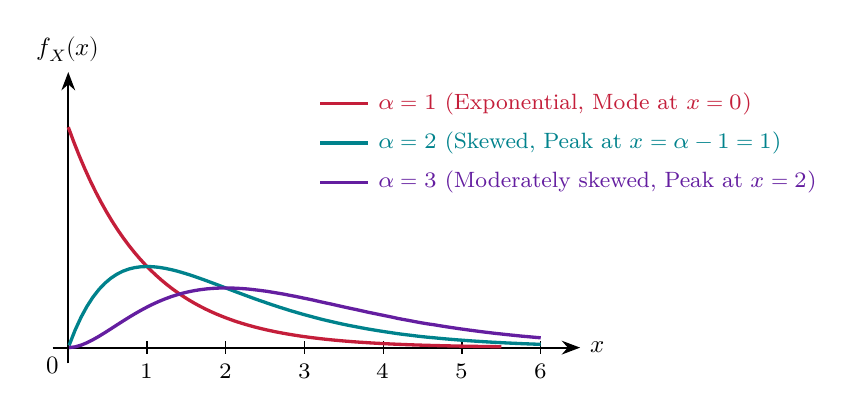
\begin{tikzpicture}[scale=1.0, every node/.style={font=\small}]
  % Axes
  \draw[-Stealth, thick] (-0.2, 0) -- (6.5, 0) node[right] {$x$};
  \draw[-Stealth, thick] (0, -0.2) -- (0, 3.5) node[above] {$f_X(x)$};

  % Ticks
  \foreach \x in {1,2,3,4,5,6} {
    \draw (\x, 0.08) -- (\x, -0.08) node[below] {\footnotesize $\x$};
  }
  \node[below left] at (0,0) {$0$};

  % alpha = 1: f(x) = e^(-x) (Exponential, monotonic decreasing)
  \draw[very thick, color=myred, domain=0:5.5, samples=80]
    plot (\x, {2.8*exp(-\x)});

  % alpha = 2: f(x) = x * e^(-x), peak at x=1 with value 1/e = 0.368 -> scaled: 2.8*0.368 = 1.03
  \draw[very thick, color=myteal, domain=0.01:6.0, samples=80]
    plot (\x, {2.8*\x*exp(-\x)});

  % alpha = 3: f(x) = (x^2 / 2) * e^(-x), peak at x=2 with value 4/(2*e^2) = 0.271 -> scaled: 2.8*0.271 = 0.76
  \draw[very thick, color=mypurple, domain=0.01:6.0, samples=80]
    plot (\x, {1.4*(\x)^2*exp(-\x)});

  % Legend
  \draw[very thick, color=myred] (3.2, 3.1) -- (3.8, 3.1) node[right, font=\footnotesize] {$\alpha = 1$ (Exponential, Mode at $x=0$)};
  \draw[very thick, color=myteal] (3.2, 2.6) -- (3.8, 2.6) node[right, font=\footnotesize] {$\alpha = 2$ (Skewed, Peak at $x = \alpha-1 = 1$)};
  \draw[very thick, color=mypurple] (3.2, 2.1) -- (3.8, 2.1) node[right, font=\footnotesize] {$\alpha = 3$ (Moderately skewed, Peak at $x = 2$)};
\end{tikzpicture}
\end{center}
\end{tcolorbox}

\newpage
% ===============================================================================
% MANDATORY QUICK REVISION PAGE
% ===============================================================================
\begin{center}
  {\large\bfseries\color{myred} Quick Revision --- Module 2}\\[1pt]
  {\small\color{mydark} Continuous Probability Distributions $|$ BS-M301}
\end{center}
\noindent{\color{myred}\rule{\linewidth}{1.0pt}}
\vspace{1pt}

\begin{tcolorbox}[formulabox, top=2pt, bottom=2pt, title={\textbf{Key Formulas and Continuous Distribution Densities at a Glance}}]
\renewcommand{\arraystretch}{0.96}
\setlength{\tabcolsep}{3.5pt}
\begin{tabularx}{\linewidth}{B{3.8cm} X}
Continuous PDF Conditions & $f_X(x) \ge 0, \quad \int_{-\infty}^\infty f_X(x) dx = 1, \quad P(a \le X \le b) = \int_a^b f_X(x) dx$ \\[0.2pt]
CDF to PDF Relationship & $F_X(x) = \int_{-\infty}^x f_X(t) dt, \quad f_X(x) = \frac{d}{dx}F_X(x), \quad P(X = c) = 0$ \\[0.2pt]
Continuous Expectation & $E[X] = \mu = \int_{-\infty}^\infty x f_X(x) dx, \quad \operatorname{Var}(X) = E[X^2] - \mu^2$ \\[0.2pt]
MGF Formula & $M_X(t) = E[e^{tX}] = \int_{-\infty}^\infty e^{tx} f_X(x) dx, \quad \mu_r' = \left.\frac{d^r M_X(t)}{dt^r}\right|_{t=0}$ \\[0.2pt]
Normal PDF $\mathcal{N}(\mu, \sigma^2)$ & $f(x) = \frac{1}{\sigma\sqrt{2\pi}} \exp\left(-\frac{(x-\mu)^2}{2\sigma^2}\right), \quad M_X(t) = \exp\left(\mu t + \frac{1}{2}\sigma^2 t^2\right)$ \\[0.2pt]
Standard Normal $Z$ & $Z = \frac{X-\mu}{\sigma} \sim \mathcal{N}(0, 1), \quad \phi(z) = \frac{1}{\sqrt{2\pi}} e^{-z^2/2}, \quad \Phi(-z) = 1-\Phi(z)$ \\[0.2pt]
Normal Moments & All odd $\mu_{2k+1} = 0, \quad \mu_2 = \sigma^2, \quad \mu_4 = 3\sigma^4, \quad \beta_1 = 0, \; \beta_2 = 3$ \\[0.2pt]
Exponential PDF $\text{Exp}(\lambda)$ & $f(x) = \lambda e^{-\lambda x} \; (x \ge 0), \quad F(x) = 1 - e^{-\lambda x}, \quad \mu = \frac{1}{\lambda}, \; \sigma^2 = \frac{1}{\lambda^2}$ \\[0.2pt]
Memoryless Property & $P(X > s+t \mid X > s) = P(X > t) \quad \text{(Unique to Exponential)}$ \\[0.2pt]
Gamma Function & $\Gamma(\alpha) = \int_0^\infty u^{\alpha-1} e^{-u} du, \quad \Gamma(\alpha+1) = \alpha \Gamma(\alpha), \quad \Gamma(1/2) = \sqrt{\pi}$ \\[0.2pt]
Gamma PDF $\text{Gamma}(\alpha, \beta)$ & $f(x) = \frac{\beta^\alpha}{\Gamma(\alpha)} x^{\alpha-1} e^{-\beta x}, \quad \mu = \frac{\alpha}{\beta}, \quad \sigma^2 = \frac{\alpha}{\beta^2}, \quad M_X(t) = \left(1-\frac{t}{\beta}\right)^{-\alpha}$ \\
\end{tabularx}
\end{tcolorbox}

\vspace{1pt}

\begin{tcolorbox}[defbox, top=2pt, bottom=2pt, title={\textbf{One-Line Definitions}}]
\begin{itemize}[leftmargin=*, itemsep=-0.5pt, topsep=0pt, parsep=0pt]
  \item \textbf{Continuous Random Variable:} Variable taking any real value in an interval, with single-point probability $P(X=c)=0$.
  \item \textbf{Probability Density Function (PDF):} Non-negative derivative of the CDF whose integral over an interval gives probability.
  \item \textbf{Normal Distribution:} Symmetrical mesokurtic bell curve fully governed by location $\mu$ and scale $\sigma$.
  \item \textbf{Inflection Points:} Points where curvature flips concavity, situated at precisely $x = \mu \pm \sigma$ for a normal curve.
  \item \textbf{Standard Score ($Z$):} Dimensionless measure $Z = (X-\mu)/\sigma$ expressing deviation from mean in units of $\sigma$.
  \item \textbf{Exponential Distribution:} Only continuous distribution possessing memorylessness, modelling Poisson inter-arrival times.
  \item \textbf{Memoryless Property:} Independence of future remaining lifetime from past survival duration: $P(X>s+t \mid X>s) = P(X>t)$.
  \item \textbf{Gamma Function ($\Gamma(\alpha)$):} Generalized factorial integral extending $n!$ to all real positive numbers ($\Gamma(n) = (n-1)!$).
  \item \textbf{Erlang Distribution:} Gamma distribution with integer shape parameter $\alpha = k$, representing sum of $k$ independent exponentials.
  \item \textbf{Reproductive Property:} Closure under convolution: sum of independent Gammas with same $\beta$ yields another Gamma.
\end{itemize}
\end{tcolorbox}

\newpage

\begin{tcolorbox}[exambox, title={\textbf{Frequently Asked / Viva Questions (Part 1)}}]
\begin{enumerate}[topsep=0pt, label=\textbf{Q\arabic*.}, itemsep=3.2pt]
  \item \Q{Why is the probability of a continuous random variable taking an exact value zero ($P(X = c) = 0$)?}
  By definition, $P(X = c) = \int_c^c f_X(x) \, dx = 0$. Since an interval contains uncountably infinitely many points, the probability mass allocated to any isolated geometric point vanishes, even though the event is not impossible in reality.

  \item \Q{Can a probability density function exceed unity ($f_X(x) > 1$)? Explain with an example.}
  Yes! Unlike discrete PMFs where $p(x) \le 1$, a continuous PDF represents probability \textit{density} per unit width, not probability. For example, for $X \sim U[0, 0.2]$, $f_X(x) = 1/(0.2 - 0) = 5.0 > 1$, while the total integral $\int_0^{0.2} 5.0 \, dx = 1.0$ is fully preserved.

  \item \Q{Derive the Moment Generating Function of the standard normal distribution $Z \sim \mathcal{N}(0, 1)$.}
  $M_Z(t) = \frac{1}{\sqrt{2\pi}} \int_{-\infty}^\infty e^{tz} e^{-z^2/2} dz = \frac{1}{\sqrt{2\pi}} \int_{-\infty}^\infty e^{-(z^2 - 2tz)/2} dz$. Completing the square: $z^2 - 2tz = (z-t)^2 - t^2$. Factoring out $e^{t^2/2}$: $M_Z(t) = e^{t^2/2} \frac{1}{\sqrt{2\pi}} \int_{-\infty}^\infty e^{-(z-t)^2/2} dz = e^{t^2/2} \cdot 1 = e^{t^2/2}$.

  \item \Q{Prove that all odd central moments of a Normal distribution are identically zero.}
  $\mu_{2k+1} = \frac{1}{\sigma\sqrt{2\pi}} \int_{-\infty}^\infty (x-\mu)^{2k+1} e^{-(x-\mu)^2/(2\sigma^2)} dx$. Substituting $u = x - \mu$: the integrand $u^{2k+1} e^{-u^2/(2\sigma^2)}$ is an odd function of $u$ ($g(-u) = -g(u)$) integrated over symmetric limits $(-\infty, \infty)$, which integrates to zero.

  \item \Q{Where do the inflection points of a normal probability curve occur?}
  Equating the second derivative to zero: $f''(x) = \left[\frac{(x-\mu)^2}{\sigma^4} - \frac{1}{\sigma^2}\right] f(x) = 0 \implies (x-\mu)^2 = \sigma^2 \implies x = \mu \pm \sigma$. The curve transitions from concave downwards to concave upwards at exactly one standard deviation on either side of the mean.

  \item \Q{State and prove the memoryless property of the Exponential distribution.}
  $P(X > s + t \mid X > s) = \frac{P(X > s + t)}{P(X > s)} = \frac{e^{-\lambda(s+t)}}{e^{-\lambda s}} = e^{-\lambda t} = P(X > t)$. The conditional probability that a component lasts $t$ more units given it has lasted $s$ units is independent of $s$.

  \item \Q{What is the physical connection between the Poisson process and the Exponential distribution?}
  In a Poisson process with rate $\lambda$, the number of event arrivals in interval $t$ follows $\text{Poisson}(\lambda t)$. The waiting time $T$ until the first arrival exceeds $t$ if and only if zero arrivals occur in $[0, t]$: $P(T > t) = P(N(t) = 0) = \frac{(\lambda t)^0 e^{-\lambda t}}{0!} = e^{-\lambda t}$. Thus, the inter-arrival time $T$ is exponentially distributed with parameter $\lambda$.
\end{enumerate}
\end{tcolorbox}

\newpage

\begin{tcolorbox}[exambox, top=3pt, bottom=3pt, title={\textbf{Frequently Asked / Viva Questions (Part 2)}}]
\begin{enumerate}[topsep=0pt, label=\textbf{Q\arabic*.}, itemsep=1.8pt, start=8]
  \item \Q{Prove that $\Gamma(1/2) = \sqrt{\pi}$.}
  $\Gamma(1/2) = \int_0^\infty u^{-1/2} e^{-u} du$. Substituting $u = z^2/2 \implies du = z dz$: $\Gamma(1/2) = \int_0^\infty \frac{\sqrt{2}}{z} e^{-z^2/2} z dz = \sqrt{2} \int_0^\infty e^{-z^2/2} dz$. By symmetry: $\int_0^\infty e^{-z^2/2} dz = \frac{1}{2} \int_{-\infty}^\infty e^{-z^2/2} dz = \frac{\sqrt{2\pi}}{2} = \sqrt{\frac{\pi}{2}}$. Multiplying by $\sqrt{2}$ yields $\Gamma(1/2) = \sqrt{\pi}$.

  \item \Q{How is the Chi-Square ($\chi^2$) distribution obtained as a special case of the Gamma distribution?}
  Setting shape parameter $\alpha = n/2$ and rate parameter $\beta = 1/2$ in the Gamma PDF yields $f(x) = \frac{(1/2)^{n/2}}{\Gamma(n/2)} x^{n/2 - 1} e^{-x/2}$, which is the standard definition of the Chi-Square distribution with $n$ degrees of freedom.

  \item \Q{State the reproductive property of independent Normal random variables.}
  If $X_1 \sim \mathcal{N}(\mu_1, \sigma_1^2)$ and $X_2 \sim \mathcal{N}(\mu_2, \sigma_2^2)$ are independent, any linear combination $Y = aX_1 + bX_2$ is also normally distributed: $Y \sim \mathcal{N}(a\mu_1 + b\mu_2, a^2\sigma_1^2 + b^2\sigma_2^2)$. This follows directly from multiplying their MGFs.
\end{enumerate}
\end{tcolorbox}

\vspace{2pt}

\begin{tcolorbox}[tikzbox, top=3pt, bottom=3pt, title={\textbf{Summary Matrix: Comprehensive Comparison of Continuous Distributions}}]
\par\vspace{1pt}\noindent
\begingroup
\setlength{\tabcolsep}{3.5pt}
\setlength{\extrarowheight}{1.0pt}
\renewcommand{\arraystretch}{1.12}
\begin{tabularx}{\linewidth}{|B{2.5cm}|B{3.8cm}|B{2.2cm}|B{2.2cm}|Y|}
\hline
\textbf{Distribution} & \textbf{Probability Density Function (PDF)} & \textbf{Mean ($E[X]$)} & \textbf{Variance ($\sigma^2$)} & \textbf{Key Engineering Application} \\
\hline
Uniform $U[a, b]$ & $f(x) = \frac{1}{b-a}, \quad x \in [a, b]$ & $\frac{a+b}{2}$ & $\frac{(b-a)^2}{12}$ & Quantization noise in ADC systems. \\
\hline
Normal $\mathcal{N}(\mu, \sigma^2)$ & $f(x) = \frac{1}{\sigma\sqrt{2\pi}} e^{-(x-\mu)^2/(2\sigma^2)}$ & $\mu$ & $\sigma^2$ & Thermal Gaussian noise; Central Limit Theorem. \\
\hline
Exponential $\text{Exp}(\lambda)$ & $f(x) = \lambda e^{-\lambda x}, \quad x \ge 0$ & $\frac{1}{\lambda}$ & $\frac{1}{\lambda^2}$ & Lifetime of electronic parts; queueing theory. \\
\hline
Gamma $(\alpha, \beta)$ & $f(x) = \frac{\beta^\alpha}{\Gamma(\alpha)} x^{\alpha-1} e^{-\beta x}, \; x > 0$ & $\frac{\alpha}{\beta}$ & $\frac{\alpha}{\beta^2}$ & Waiting time for $\alpha$ events; reliability engineering. \\
\hline
Chi-Square $\chi^2(n)$ & $f(x) = \frac{(1/2)^{n/2}}{\Gamma(n/2)} x^{n/2-1} e^{-x/2}$ & $n$ & $2n$ & Goodness-of-fit testing; sample variance distribution. \\
\hline
\end{tabularx}
\endgroup
\end{tcolorbox}

\end{document}
